%! TeX program = lualatex
\documentclass[../main.tex]{subfiles}

\usetikzlibrary{intersections,calc}

\newenvironment{solution}{
  \begin{proof}[Sample solution]
    \color{main}
  }{
  \end{proof}
}

\begin{document}

\chapter*{Week 9 practice problems}

\setcounter{chapter}{9}

\begin{exercise}
  Consider the following probability mass function for a discrete random variable \(X\).
  \[
    f(x) =
    \begin{cases}
      0.05, & x = 1,\\
      0.10, & x = 2,\\
      0.15, & x = 3,\\
      0.20, & x = 4,\\
      0.10, & x = 5,\\
      0.15, & x = 6,\\
      0.05, & x = 7,\\
      0.10, & x = 8,\\
      0.10, & x = 9,\\
      0, & \text{otherwise}.
    \end{cases}
  \]

  \begin{multicols}{2}
    \begin{enumerate}
      \item Sketch its PMF.
      \item Write down its cumulative distribution function \(F(x)\).
      \item Sketch its CDF.
      \item Calculate \(\mathbb{P}(3 < X \le 5)\).
      \item Calculate \(\mathbb{P}(2 \le X < 9)\).
      \item Calculate \(\mathbb{P}(4 \le X \le 6)\).
      \item Calculate \(\mathbb{P}(X \le 6)\).
      \item Calculate \(\mathbb{P}(X < 3)\).
      \item Calculate \(\mathbb{P}(X \ge 4)\).
      \item Calculate \(\mathbb{P}(X \ge 4)\).
      \item Calculate its expectation, variance and standard deviation.
    \end{enumerate}
  \end{multicols}

\end{exercise}

\begin{exercise}
  Consider the following cumulative distribution function for a discrete random variable \(X\).
  \[
    F(x) =
    \begin{cases}
      0.00, & x < -5, \\[4pt]
      0.07, & -5 \le x < -3, \\[4pt]
      0.18, & -3 \le x < -2, \\[4pt]
      0.29, & -2 \le x < 0, \\[4pt]
      0.43, & 0 \le x < 1, \\[4pt]
      0.61, & 1 \le x < 2, \\[4pt]
      0.72, & 2 \le x < 4, \\[4pt]
      0.85, & 4 \le x < 7, \\[4pt]
      0.93, & 7 \le x < 10, \\[4pt]
      1.00, & x \ge 10.
    \end{cases}
  \]

  \begin{multicols}{2}
    \begin{enumerate}
      \item Sketch its CDF.
      \item Write down its probability mass function function \(F(x)\).
      \item Sketch its PMF.
      \item Calculate \(\mathbb{P}(3 < X \le 5)\).
      \item Calculate \(\mathbb{P}(2 \le X < 9)\).
      \item Calculate \(\mathbb{P}(4 \le X \le 6)\).
      \item Calculate \(\mathbb{P}(X \le 6)\).
      \item Calculate \(\mathbb{P}(X < 3)\).
      \item Calculate \(\mathbb{P}(X > 5)\).
      \item Calculate \(\mathbb{P}(X \ge -2)\).
      \item Calculate its expectation, variance and standard deviation.
    \end{enumerate}
  \end{multicols}
\end{exercise}

\begin{exercise}
  Sketch the PMF for the given discrete random variable \(X\).  Estimate \(\mathbb{P}(-3 < X \le 8)\) and \(\mathbb{P}(X = -1)\).  Without any calculations, estimate its expectation.
  \begin{center}
    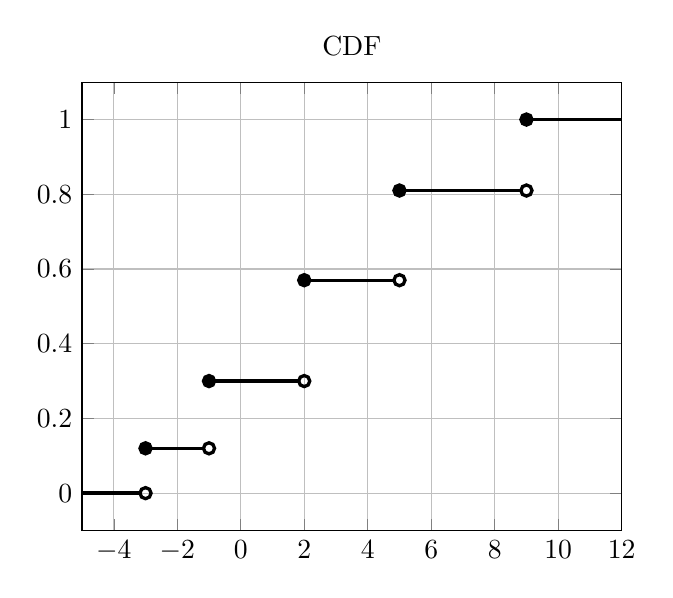
\begin{tikzpicture}
      \begin{axis}[grid=major, title={CDF}, xmin=-5, xmax=12, ytick={0,0.2,0.4,0.6,0.8,1}, ymin=-0.1, ymax=1.1]
        \addplot[very thick, black] coordinates { (-5,    0) ({-3 - 0.20}, 0.00)  };
        \addplot[very thick, black] coordinates { (-3, 0.12) ({-1 - 0.20}, 0.12)  };
        \addplot[very thick, black] coordinates { (-1, 0.30) ({ 2 - 0.20}, 0.30) };
        \addplot[very thick, black] coordinates { ( 2, 0.57) ({ 5 - 0.20}, 0.57) };
        \addplot[very thick, black] coordinates { ( 5, 0.81) ({ 9 - 0.20}, 0.81) };
        \addplot[very thick, black] coordinates { ( 9, 1.00) ({13 - 0.20}, 1.00)  };
        \addplot[very thick, only marks, mark=o] coordinates {
            ({-3 - 0.00}, 0.00)
            ({-1 - 0.00}, 0.12)
            ({ 2 - 0.00}, 0.30)
            ({ 5 - 0.00}, 0.57)
            ({ 9 - 0.00}, 0.81)
          };
        \addplot[very thick, only marks, mark=*] coordinates {
            (-3, 0.12)
            (-1, 0.30)
            ( 2, 0.57)
            ( 5, 0.81)
            ( 9, 1.00)
          };
      \end{axis}
    \end{tikzpicture}
    \qquad
    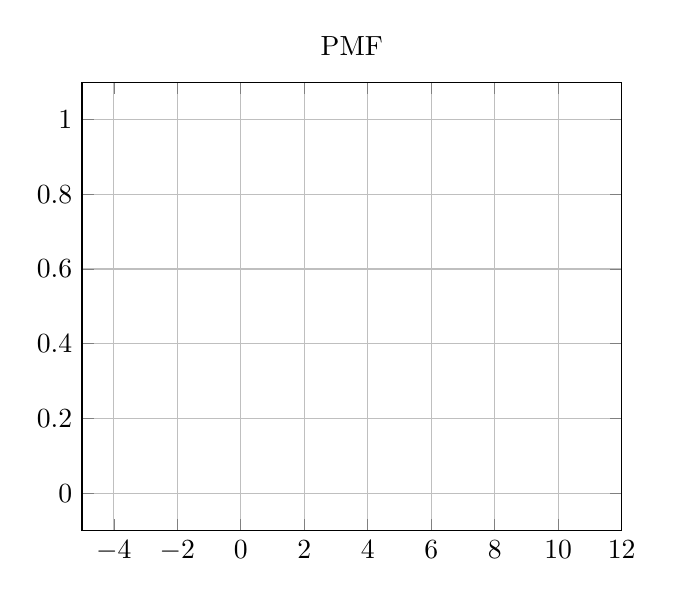
\begin{tikzpicture}
      \begin{axis}[grid=major, title={PMF}, xmin=-5, xmax=12, ytick={0,0.2,0.4,0.6,0.8,1}, ymin=-0.1, ymax=1.1]
        \addplot[opacity=0] coordinates {(-5, 0.2) (12,0.2)};
        % \addplot[very thick, black] coordinates { (-4,    0) ({-3 - 0.20}, 0.00)  };
        % \addplot[very thick, black] coordinates { (-3, 0.12) ({-1 - 0.20}, 0.12)  };
        % \addplot[very thick, black] coordinates { (-1, 0.30) ({ 2 - 0.20}, 0.30) };
        % \addplot[very thick, black] coordinates { ( 2, 0.57) ({ 5 - 0.20}, 0.57) };
        % \addplot[very thick, black] coordinates { ( 5, 0.81) ({ 9 - 0.20}, 0.81) };
        % \addplot[very thick, black] coordinates { ( 9, 1.00) ({13 - 0.20}, 1.00)  };
        % \addplot[very thick, only marks, mark=o] coordinates {
        %     ({-3 - 0.00}, 0.00)
        %     ({-1 - 0.00}, 0.12)
        %     ({ 2 - 0.00}, 0.30)
        %     ({ 5 - 0.00}, 0.57)
        %     ({ 9 - 0.00}, 0.81)
        %   };
        % \addplot[very thick, only marks, mark=*] coordinates {
        %     (-5,    0)
        %     (-3, 0.12)
        %     (-1, 0.30)
        %     ( 2, 0.57)
        %     ( 5, 0.81)
        %     ( 9, 1.00)
        %   };
      \end{axis}
    \end{tikzpicture}
  \end{center}
\end{exercise}

\begin{exercise}
  Consider the following probability density function for a continuous random variable.
  \[
    f(x) =
    \begin{cases}
      \dfrac{2}{9} (x - 2), & 2 \le x \le 5, \\[6pt]
      0, & \text{otherwise}.
    \end{cases}
  \]

  \begin{enumerate}
    \item Find its cumulative distribution function.
    \item Calculate its expectation, variance and standard deviation.
  \end{enumerate}
\end{exercise}

\begin{exercise}
  The probability density function for a continuous random variable \(X\) is given below.
  \[
    f(x) =
    \begin{cases}
      \dfrac{1}{2} x, & 0 \le x \le 1, \\[8pt]
      \dfrac{1}{2}(2x - 4), & 2 \le x \le 3, \\[8pt]
      \dfrac{1}{2}(6 - x), & 5 \le x \le 6, \\[8pt]
      0, & \text{otherwise}.
    \end{cases}
  \]

  \begin{enumerate}
    \item Find its cumulative distribution function.
    \item Calculate \(\mathbb{P}(1/2 \le X < 5.5)\).
    \item Calculate its expectation, variance and standard deviation.
  \end{enumerate}
\end{exercise}

\begin{exercise}
  Consider the probability density functions below. Which continuous random variables has a higher standard deviation? Which has a higher expectation? Which has a higher variance?

  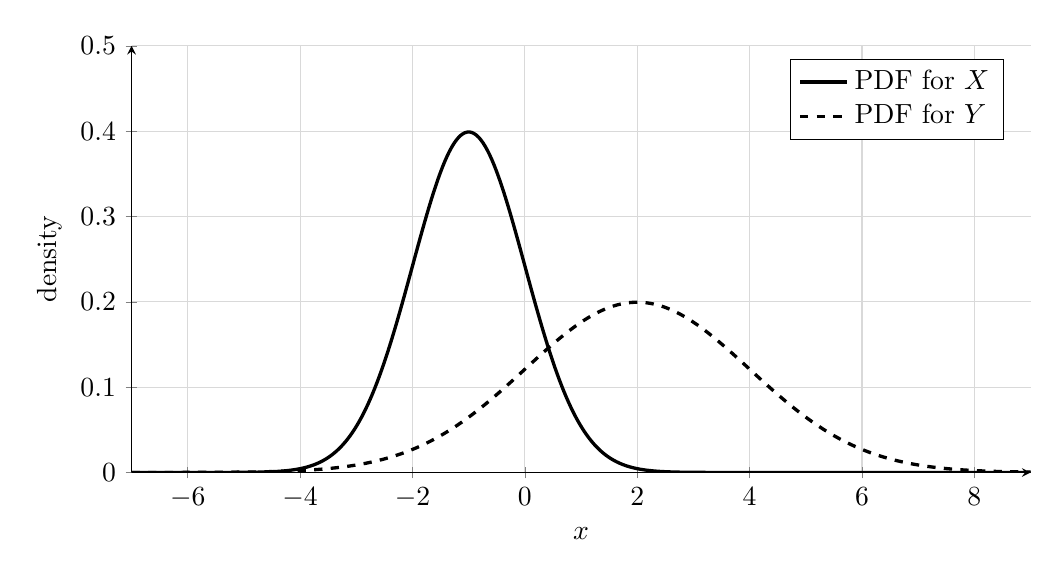
\begin{tikzpicture}
    \begin{axis}[
      width=13cm, height=7cm,
      axis lines=left,
      xlabel={$x$},
      ylabel={density},
      xmin=-7, xmax=9,
      ymin=0, ymax=0.5,
      grid=both,
      minor grid style={gray!15},
      major grid style={gray!30},
      legend cell align=left,
      legend pos=north east,
      domain=-7:9,
      samples=400
      ]

      % N(-1, 1)
      \addplot[very thick]
        ({x}, { (1.0/sqrt(2*pi*1^2)) * exp(-(x - (-1))^2 / (2*1^2)) });
      \addlegendentry{PDF for \(X\)};

      % N(2, 2)
      \addplot[very thick, dashed]
        ({x}, { (1.0/sqrt(2*pi*2^2)) * exp(-(x - 2)^2 / (2*2^2)) });
      \addlegendentry{PDF for \(Y\)};

    \end{axis}
  \end{tikzpicture}
\end{exercise}

\begin{exercise}
  The probability density function of a continuous random variable is given below. Find the unknown constant \(a\).

  \[
    f(x) =
    \begin{cases}
      a x, & 0 \le x \le 2, \\[8pt]
      0.35\, (6 - x), & 4 \le x \le 6, \\[8pt]
      0, & \text{otherwise}.
    \end{cases}
  \]
\end{exercise}

\begin{exercise}
  The graph of a function \(f(x)\) is given. Is it a valid PDF for a continuous random variable? If so, sketch its cumulative distribution function. Try to do so without any calculations.

  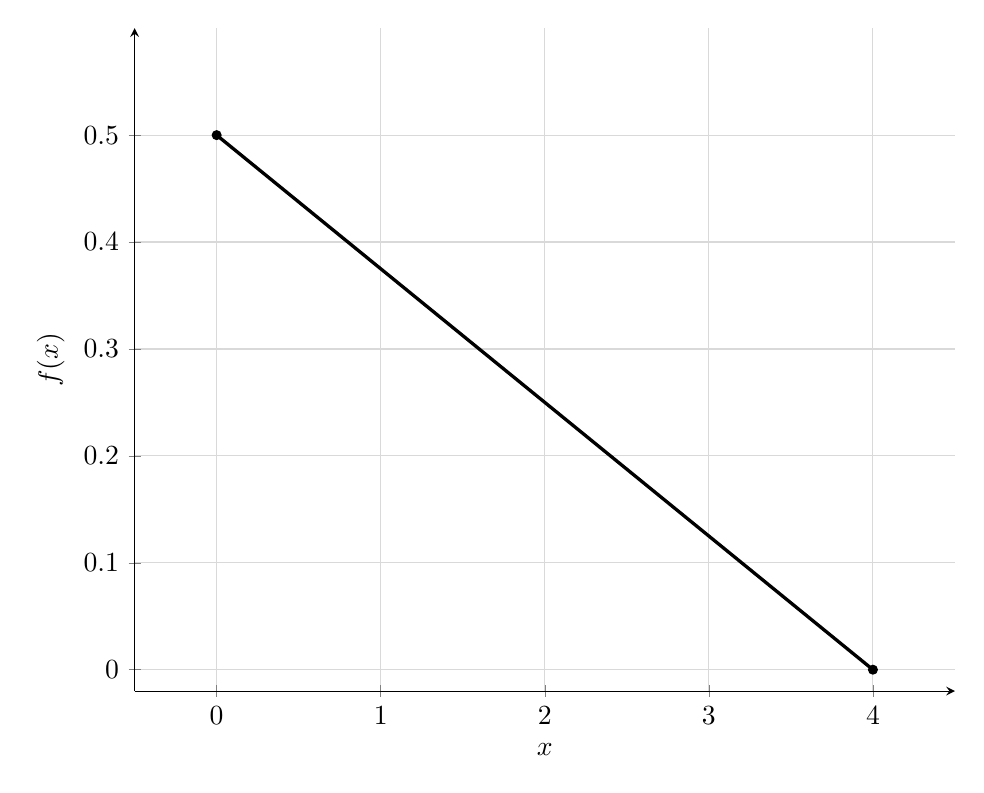
\begin{tikzpicture}
    \begin{axis}[
      width=12cm, height=10cm,
      axis lines=left,
      xlabel={$x$},
      ylabel={$f(x)$},
      xmin=-0.5, xmax=4.5,
      ymin=-0.02, ymax=0.6,
      grid=both,
      minor grid style={gray!15},
      major grid style={gray!30},
      xtick={0,1,2,3,4},
      ytick={0,0.1,0.2,0.3,0.4,0.5},
      domain=0:4,
      samples=2  % straight line between the two endpoints
      ]

      % f(x) = (1/8)(4 - x) on [0,4]
      \addplot[very thick] {(1/8)*(4 - x)};

      % Optional: emphasize endpoints on the support
      \addplot[only marks, mark=*, mark size=1.6pt] coordinates {(0,0.5) (4,0)};

    \end{axis}
  \end{tikzpicture}
\end{exercise}
\clearpage

\begin{exercise}
  Tommy's sells mystery donut boxes. Each box is supposed to weigh the same but may contain a different number of donuts.  Over the course of a semester, someone weighed every single donut they bought and recorded the following data.  If the next 10 donuts they buy all weigh around \(15\) to \(20\) grams, how do you expect the expectation to change?

  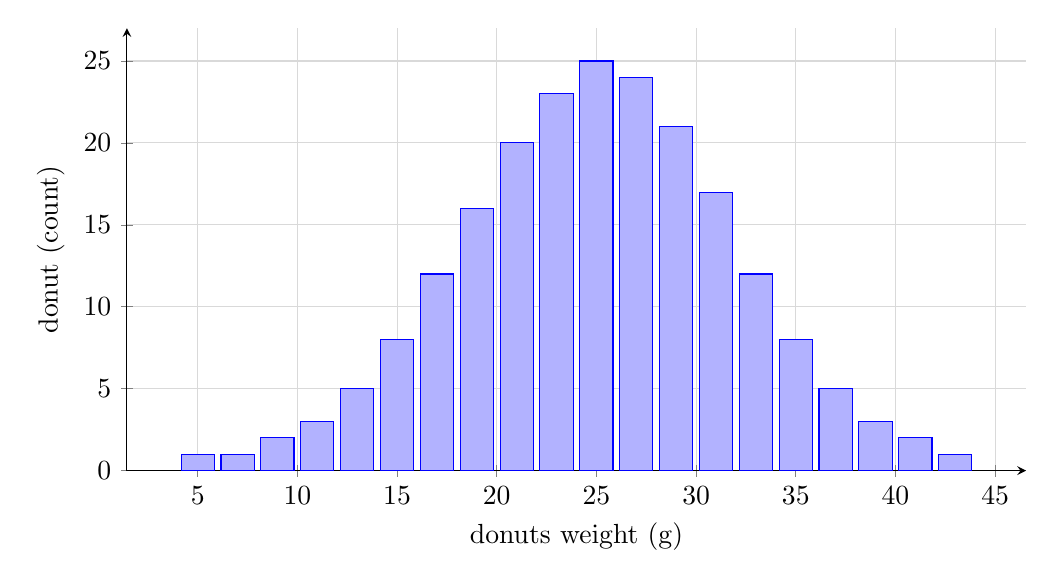
\begin{tikzpicture}
    \begin{axis}[
      width=13cm, height=7.2cm,
      ybar,
      bar width=12pt,
      axis lines=left,
      xlabel={donuts weight (g)},
      ylabel={donut (count)},
      xmin=3.5, xmax=44.5,
      ymin=0, ymax=27,
      % xtick={5,7,9,11,13,15,17,19,21,23,25,27,29,31,33,35,37,39,41,43},
      ytick={0,5,10,15,20,25},
      enlarge x limits=0.05,
      grid=both,
      minor grid style={gray!15},
      major grid style={gray!30},
      legend pos=north east,
      legend cell align=left
      ]

      % 20-bin histogram of cracked donuts by weight.
      % Bins (centers): 5, 7, ..., 43 (step = 2 g)
      % Counts chosen to be bell-shaped around 25 g, with peak = 25.
      % Feel free to tweak these to change the "random" look while keeping the shape.
      \addplot coordinates {
          (5,1) (7,1) (9,2) (11,3) (13,5)
          (15,8) (17,12) (19,16) (21,20) (23,23)
          (25,25) (27,24) (29,21) (31,17) (33,12)
          (35,8) (37,5) (39,3) (41,2) (43,1)
        };

    \end{axis}
    \end{tikzpicture}
\end{exercise}

\begin{exercise}
  Which of the following statements are true for a probability density function \(f(x)\) of a continuous random variable \(X\)?

  \begin{enumerate}
    \item \(f(x)\) is never decreasing.
    \item \(f(x)\) is allays increasing.
    \item \(E(X)\) is always positive.
    \item Variance is the square root of standard deviation.
    \item Standard deviation can be negative.
    \item \(\lim_{x \to \infty} f(x) = 1\).
    \item If \(f(x)\) is positive over \([3, 10]\), then \(f(x) \le 1/7\) over \([3,10]\).
  \end{enumerate}
\end{exercise}

\begin{exercise}
  A game is played by flipping a fair coin three times. Each time heads is flipped, you receive one cookie. Each time tails is flipped you receive \(5\) cookies. You play this game once.

  Model the game using a random variable.

  \begin{enumerate}
    \item List all outcomes of the underlying sample space of \(X\).
    \item Describe the probability mass function for \(X\).
    \item Find \(E(X)\).
  \end{enumerate}
\end{exercise}
\end{document}
